\chapter{Functional Objectives and Exisiting Solutions}

\section{Usage Scenarios}
TODO introductions

\subsection{Asking for Help}
Having the possibility to ask for help is a vital part of knowledge driven
businesses, so collaboration and the sharing of ideas are a major factor in the company guidelines
of SinnerSchrader. The application should act as a central repository for knowledge and contacts,
enabling employees to find someone who can help in order to solve questions and find solutions faster.

\subsection{Finding Potential Team Members}
Team managers constantly face the problem of reassembling parts of their teams, forming new teams for new projects, and
disbanding teams whose projects have ended. As there is no unified source of information about all employees, managers often
do not find the best suitable team member to fill an open position because they simply do not know each other yet.
The tool will give managers the opportunity to search the entirety of employees at SinnerSchrader and find one
meeting all requirements of the open position, thus making collocating teams easier and more efficient.

\subsection{Collecting Information}
The application will give employees the possibility to provide information about their personal knowledge regarding the
skills known by the application. Furthermore, they can assign a will value for every skill that describes if they prefer
doing the implicitly linked activity or working with the tool described by said skill. That is, people can define what they want to do and what tasks they would like to refuse.\\
As employees continually enlarge their knowledge while their fields of interest shift towards new technologies, tools or even
functional divisions, providing data about their skills and preference once will lead to the system being filled with obsolete
information. The quality of the applications search results and suggestions heavily relies on the fidelity and volume of the underlying data about the employees, hence keeping said information up to date is crucial to the performance of the application.

\subsubsection{Biannual Feedback Meetings}
Every employee has biannual meetings with their respective supervisor to interchange
bidirectional feedback, define personal goals, and negotiate possible changes of salary.
Part of the feedback given by the employee are subjects their learned or enhanced their knowledge about, and newly developed interests. These insights are documented and registered in the employee's personnel file.
This meeting will be the regular occasion for supervisors and employees to refine the data saved in the application and to add
newly gained skills to it. The supervisor is advised to address discrepancies between the employee's and their own estimations of skills.

\subsection{Notifications by Supervisors}
Employees and supvervisors are encouraged to be in rich contact with each other in order to deliver continous feedback
about the individual person's needs, impediments, and the status of their current projects.
As a result, supervisors can identify appropriate moments for reevaluating the skills and preferences saved in the application and notify the employee.\\
For example, according to Tuckman's team development model, the so called `adjourning' phase of a project is an occasion for `recognition of individual achievements and reflection on how far the team has come' \cite[P. 3]{Wilson} and thus is a convenient chance to add new skills acquired during the project and to refine the existing data.

\subsubsection{Automatic Notifications}
TODO write warum nicht

\subsubsection{Intrinsic Motivations}
In addition to the mentioned reasons for employees to provide data about their skills which are all extrinsic motivations,
there also exist intrinsic motivations to do so. Being motivated intrinsically can be defined as `doing something because it is inherently interesting or enjoyable' \cite{RYAN200054}. As people are motivated to focus on tasks they fancy, they are also motivated to voluntarily keep an eye on the quality of the data that is used to determine the tasks they will have to perfom.


\subsection{Rating Colleagues}
TODO
keine Motivation
BR sagt nein



\section{Requirements}
\subsection{Functional Requirements}
\begin{itemize}
  \item TODO: usable to all
	\item User Profiles \\
	Anyone can see another user’s profile consisting of basic information about the user such as Name, Location, E-Mail and personal skills. Personal skills are composed of a name, a knowledge level and a will level, both on a scale from one to four.
	\item Provide/Edit skills\\
	Users can add new skills from a pool of known skills to their own profile. Already added skills can be edited and removed from the profile.
	\item Search\\
	A search function can be used to find people who have added one or more specific skills to their profile. When searching for multiple skills, only persons matching all of them will will be displayed.
	\begin{itemize}
		\item Ranking\\
			By default, the search results order should be defined by a score aggregating the individual employee's skill level, will level and grade of spezialization in the searched skills. Employees willing to enhance their knowledge about a searched skill should be preferred to others having the same knowledge but a lower will.
		\item Sorting\\
			The user should be able to sort the search results not only by said score,
			but also solely by knowledge and will level.
	\end{itemize}
	\item Management of known skills\\
	New skills can be added to the set of known skills in the application. Existing skills can be edited and removed. Users personal skills are automatically updated when a skill has been edited so that the integrity of the user profiles is maintained at all times.
\end{itemize}

\subsection{Non Functional Requirements}
TODO: Klären und formulieren
\begin{itemize}
	\item Desktop/Devices
	\item Browsers
	\item Scalability
	\item Load/Response Times
\end{itemize}



\section{Commercial Solutions}
TODO Bla bla Stichprobe

\subsection{Skills Base}
Skills Base\footnote{http://http://www.skills-base.com/} offers the required features, but also includes a large number of functionality SinnerSchrader does not need and ist not willing to use. This includes assessments, the categorization of skills and a role model for advanced access rights configuration.
The search function does not provide searching for multiple skills. Furthermore, the sorting of results found cannot be customized. A central point of the application are dashboards displaying information about the most popular skills in the organisation and long term statistics.
\begin{figure}[!htp]
    \centering
    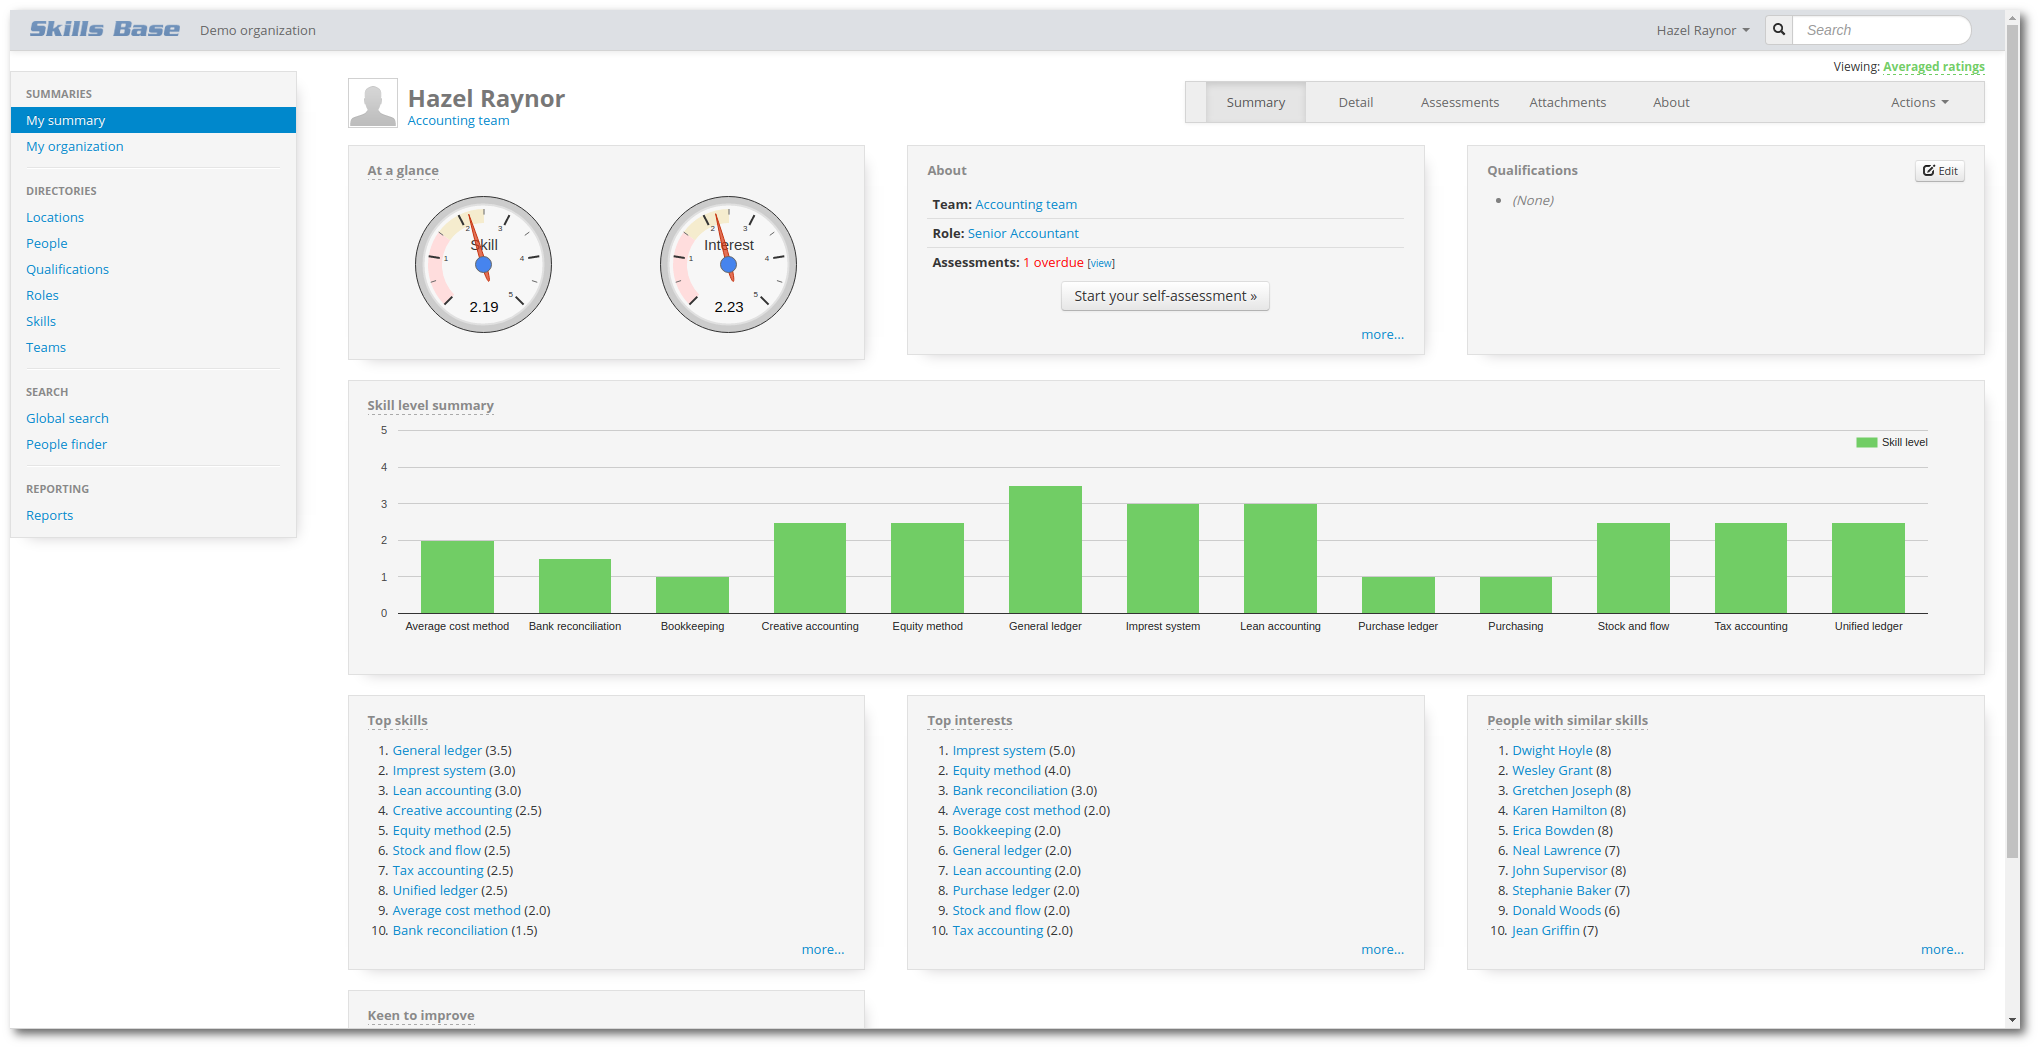
\includegraphics[width=0.8\textwidth]{images/skillsbase-dashboard.png}
    \caption{SkillsBase Dashboard}
    \label{fig:skillsbase_dashboard}
\end{figure}

\subsection{Talent Management (engage!)}
Talent Management\footnote{http://www.infoniqa.com/hr-software/skill-management} is a module for Infoniqa’s management software engage!. It offers advanced features for managers such as a powerful search function controlled via a special query language. It also includes data about the employees’ salaries, feedback protocols and certificates. It can only be used in combination with engage!, an complete human resources management solution including features like time tracking, e-learning, applicant management and payroll accounting.

\begin{figure}[!htp]
    \centering
    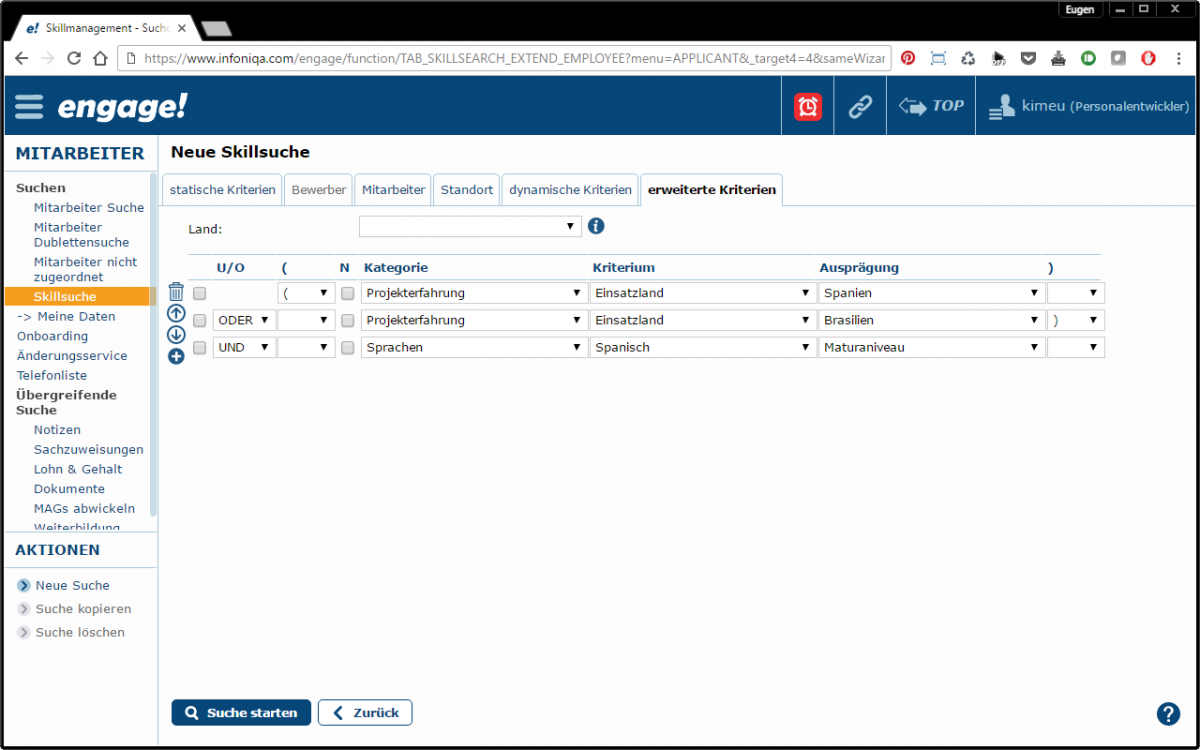
\includegraphics[width=0.8\textwidth]{images/talent_management_-_skillmanagement_-_skillsuche.png}
    \caption{Talent Management Search}
    \label{fig:talent_management}
\end{figure}

\subsection{SkillsDB Pro}
SkillsDB Pro\footnote{http://www.skillsdbpro.com} is an application designed to serve as a database in an organization providing an overview about every person’s own skills and and trainings only to themselves and their manager. The search function is capable of searching for multiple skills combined with different logical operators which enables users to enter very sophisticated queries.
Not only can users provide information about their skills, but managers can also do this with the limitation that no employee can see their manager’s rating about themselves.
Furthermore, only managers can search for persons. Taking into consideration that SinnerSchrader needs a tool to enable everyone to find someone with a specific skillset, this is a serious disadvantage.
SkillsDB also offers features SinnerSchrader does not intent to use including, but not limited to the automatic generation of project reports based on plan succession and demands for assessments.

\subsection{Conclusion}
None of the analyzed softwares offers all features required, but all of them include various functions SinnerSchrader does not intend to use, which brings undesired complexity into the applications.
One of the most critical features, sorting the search results by best match, is not offered by any of the commercial solutions.
Furthermore, all those systems differentiate between employees and their supervisors and thus restrain transparency. Instead of a solution for monitoring employees and rating them, we want a tool for everyone to find another person who offers the skills needed to solve a concrete problem.

\subsubsection{Pain Point Fitness Scoring}
As shown by \cite{CanosDaros2013}, motivation is a vital factor regarding any employee's performance and quality of work.
Although motivation is a complex construct of many highly diverse dimensions, the overlap of a person's interests and their duties is a key aspect to it.
Assuming that every member of the company has some skills they prefer to employ over others, matching people to tasks that require the exact same abilities they are interested in employing will lead to more motivated employees and thus have a positive impact on the overall productivity of SinnerSchrader.
Consequentely, when searching for persons having specific skills, the application should not only take into acount the employees' skills but only their preferences in order not to find the most skilled, but the best fitting one. Unfortunally, none of the examined applications does provide a way to aggregate both, skills and preferences, into a
single score indicating the overall grade suitability of a person relative to the searched skills.
